\subsection{Tracing Oscillations through the Learned Function}
\label{subsec:tracing}

A parameter update changes the representations computed inside the
network and, eventually, its output. We trace these changes backwards
from the output toward the input-side layers, asking where they reverse,
how large they become, and whether different parts of the network share
their timing. We compare the same inputs at successive training states;
otherwise, a representation difference could arise simply because the
examples changed. The reference sets are all 5,000 MLP training images,
one original 1,000-image ResNet normalization group, and 64 Transformer
sequences with 2,240 unchanged token positions (Table~\ref{tab:setup}).

A training state $\theta_t$ is the parameter state after $t$ completed
updates. For a window $a{:}b$, we analyze the $T_w=b-a+1$ representation
changes ending at steps $a,\ldots,b$. Computing their consecutive
cosines requires states $a-2,\ldots,b$: the first cosine compares the
changes ending at $a-1$ and $a$.

A measured \emph{site} is a named output in the computation graph.
It can be a single layer, an attention module, or the end of a residual
block group; we record that output rather than averaging internal layers.
Write its activation matrix as $A_t^\ell\in\mathbb R^{N_\ell\times m_\ell}$.
The $N_\ell$ rows identify reference examples and, where relevant, spatial or token
positions; columns identify the $m_\ell$ features at each position.
The preceding update changes this representation by
\begin{equation}
 \delta_t^\ell=\operatorname{vec}(A_t^\ell-A_{t-1}^\ell)
 \in\mathbb R^{P_\ell},\qquad P_\ell=N_\ell m_\ell.
 \label{eq:representation-change}
\end{equation}
Each flattened coordinate is one feature's response at one matching
input position. No examples or features are averaged before measuring
the change. Its direction and size are measured using
\begin{equation}
 c_t^\ell=
 \frac{\langle\delta_{t-1}^\ell,\delta_t^\ell\rangle}
 {\|\delta_{t-1}^\ell\|\|\delta_t^\ell\|},\qquad
 a_t^\ell=\frac{\|\delta_t^\ell\|}{\sqrt{P_\ell}}.
 \label{eq:representation-motion}
\end{equation}
A negative $c_t^\ell$ means the new functional change opposes the
preceding one; positive values indicate reinforcement. As $\rho_t$ measures alignment between consecutive raw gradients,
$c_t^\ell$ measures alignment between consecutive functional changes at
site $\ell$, giving a representation counterpart of constructive and
destructive regimes. The root-mean-square (RMS) displacement $a_t^\ell$
measures the change per coordinate. A zero change has undefined cosine.

The representation counterpart of normalized displacement is
\begin{equation}
 R_{a:b}^\ell=
 \frac{\|\sum_{t=a}^b\delta_t^\ell\|}{\sum_{t=a}^b\|\delta_t^\ell\|}
 =\frac{\|A_b^\ell-A_{a-1}^\ell\|_F}
 {\sum_{t=a}^b\|A_t^\ell-A_{t-1}^\ell\|_F}.
 \label{eq:representation-retention}
\end{equation}
This ratio lies in $[0,1]$ whenever movement occurs: it compares net
displacement with total distance traveled. In the windows below, output
retention is only 1.71\%/2.44\%/3.51\% for MLP/ResNet/Transformer;
the first measured sites retain 3.25\%/3.72\%/24.33\%, respectively.
Together with negative cosines, these values show substantial
back-and-forth movement with little remaining net displacement,
motivating control of its magnitude. Retention measures displacement,
rather than learning quality; orthogonal changes can also produce a
small ratio. All values use the full changes, without mode truncation.

For each site separately, collect the
changes at steps $a,\ldots,b$ into
$D_\ell\in\mathbb R^{T_w\times P_\ell}$, where $T_w=b-a+1$.
Each row is $(\delta_t^\ell)^\top$, and each column follows one fixed
input-position/feature coordinate across updates. A single singular
value decomposition (SVD) fits the whole window,
\begin{equation}
 D_\ell=U_\ell\Sigma_\ell V_\ell^\top.
 \label{eq:temporal-svd}
\end{equation}
The columns $v_{\ell,j}$ of $V_\ell$ are orthonormal patterns of
representation change. A pattern specifies which coordinates change
together and in what proportions. Its coefficient varies in magnitude
and sign from one update to the next. The diagonal entries
$\sigma_{\ell,j}$ of $\Sigma_\ell$ are nonnegative singular values,
ordered from largest to smallest, and $U_\ell$ describes their temporal
variation. Specifically,
\begin{equation}
 \delta_t^\ell=\sum_j\alpha_{t,j}^\ell v_{\ell,j},\qquad
 \alpha_{t,j}^\ell=\sigma_{\ell,j}U_{\ell,(t-a+1),j}.
 \label{eq:pattern-reconstruction}
\end{equation}
A \emph{mode} is the right singular vector
$v_{\ell,j}\in\mathbb R^{P_\ell}$: the $j$th fixed pattern at site $\ell$
over the whole window. Its coordinates span all reference input positions
and features; its indices identify the site and pattern, not a sample
or training step. Equivalently, it is an eigenvector of
$D_\ell^\top D_\ell$ with eigenvalue $\sigma_{\ell,j}^2$.
The rectangular matrix $D_\ell$ itself need not have eigenvectors.
At most $\min(T_w,P_\ell)$ independent patterns can be observed.

The total squared movement is $\|D_\ell\|_F^2=\sum_j\sigma_{\ell,j}^2$.
The fraction captured by the first $k$ patterns is
\begin{equation}
 E_k^\ell=\frac{\sum_{j=1}^k\sigma_{\ell,j}^2}
 {\sum_j\sigma_{\ell,j}^2}.
 \label{eq:energy}
\end{equation}
Thus $E_k^\ell=0.95$ means that reconstruction using these $k$ patterns
retains 95\% of squared movement, leaving 5\% squared reconstruction
error. This quantity is often called cumulative energy, with
``cumulative'' referring to patterns, not steps. We use squared movement
instead of variance because the change matrix is not centered: a
persistent drift is part of the movement being measured. Row norms are
also retained, so larger changes contribute more.

To compare timing across sites of different widths, we compare the
columns of $U_\ell$, whose coordinates always index the same training
steps. Write $U_{\ell,k}$ for the first $k$ columns of $U_\ell$. With $F$ denoting the final network output, their leading-$k$ overlap is
\begin{equation}
 O_k(\ell,F)=\frac{\|U_{\ell,k}^{\top}U_{F,k}\|_F^2}{k}.
 \label{eq:overlap}
\end{equation}
It measures how much of a site's leading time histories lies in the
subspace spanned by the final output's leading time histories. A value of one means the same temporal subspace,
even if the individual basis vectors differ; zero means orthogonal
temporal subspaces. We use $k=10$ within the numerical ranks. This measures shared timing, without backpropagating outputs or
equating feature directions at different sites.

Algorithm~\ref{alg:trace} assembles these measurements.

\begin{algorithm}[H]
\caption{Tracing representation changes through a network}
\label{alg:trace}
\begin{algorithmic}[1]
\Require Training trajectory; ordered reference examples; measured sites; window $a{:}b$
\State Evaluate the same examples at states $a-2,\ldots,b$, preserving normalization groups and training state.
\For{each measured site $\ell$}
 \State Compute consecutive activation differences $\delta_t^\ell$.
 \State Measure change cosine $c_t^\ell$ and RMS displacement $a_t^\ell$; align them with loss at step $t$.
 \State Stack changes $a{:}b$ as rows of $D_\ell$ and compute $R_{a:b}^\ell$.
 \State Decompose $D_\ell D_\ell^\top$ to obtain movement energies and signed coefficient histories.
\EndFor
\State Compute temporal overlap $O_k(\ell,F)$ with the final network output.
\State Analyze the raw gradients used by the same updates separately.
\end{algorithmic}
\end{algorithm}

\begin{figure*}[!t]
\centering
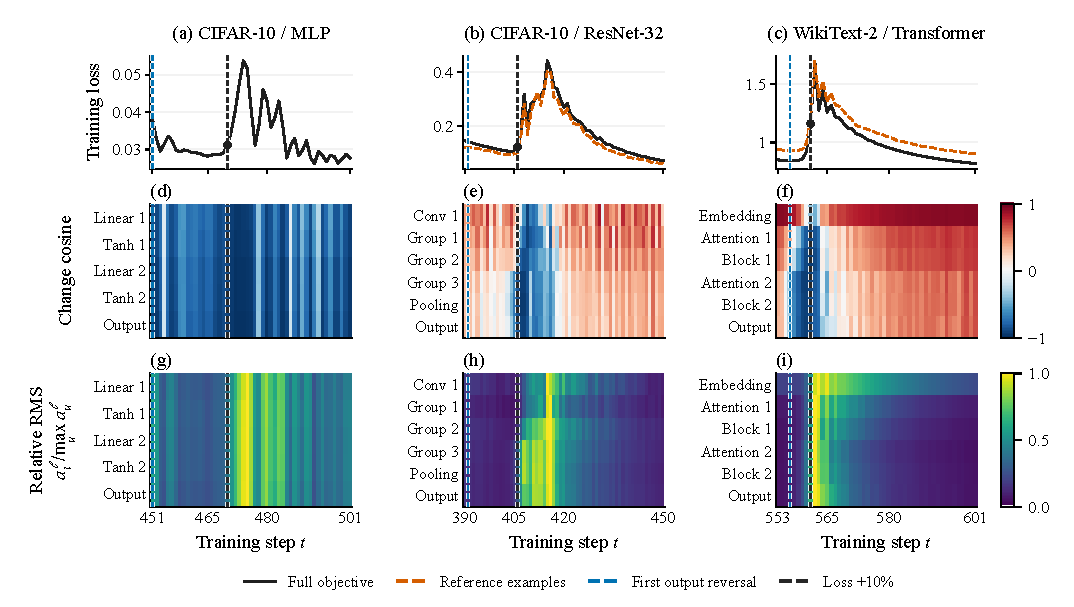
\includegraphics[width=\textwidth]{figures/00-three-model-loss-representation-motion.pdf}
\caption{Loss and representation changes in selected Adam windows: steps 451--501 (MLP), 390--450 (ResNet), and 553--601 (Transformer). Top: complete training loss and loss on the reference examples. Middle: cosine between consecutive representation changes; blue denotes reversal and red denotes reinforcement. Bottom: relative RMS displacement $a_t^\ell/\max_{u\in[a,b]}a_u^\ell$, normalized separately within each site and displayed window. The 5/6/6 rows are measured site outputs, not averages of internal layers. Reference sets contain 5,000 images, one original 1,000-image BatchNorm group, and 2,240 token positions. Blue dashed lines mark the first displayed negative output-change cosine; the MLP is already negative at entry. Black dashed lines mark the first loss at least 10\% above the pre-peak minimum. These lines compare timing; they do not identify a unique initiating event.}
\label{fig:trace-motion}
\end{figure*}

Figure~\ref{fig:trace-motion} shows where functional oscillation appears
and how its size changes. The top row locates the loss excursion.
Reading the cosine maps backwards from output to input reveals how
widely reversal is shared. In the MLP, every displayed change has
negative cosine at every measured site, from the first linear input
map to the final output. Oscillation is therefore homogeneous across
the measured depth, even while loss rises and falls. The RMS maps add
its changing amplitude. Comparing pre- and post-nonlinearity measurements
shows that tanh attenuates displacement; each site's separate
normalization in the figure highlights timing rather than absolute
differences in magnitude across sites.

ResNet and Transformer exhibit a less homogeneous pattern. Their
output-side representations reverse while earlier representations can
continue to reinforce their preceding change. The first displayed output
reversal precedes the 10\% loss marker by 15 steps in ResNet and five
in Transformer. In ResNet, the first convolution reaches its largest
displacement at the loss peak, followed one step later by the remaining
displayed sites. In Transformer, the embedding becomes more oscillatory
near the large excursion and returns to constructive movement sooner
than the later sites. Larger backpropagated errors could recruit earlier
representations into stronger changes, while constructive intervals
could accumulate smaller changes before that reorganization. This
architecture-dependent interpretation motivates examining both the
direction and magnitude throughout the network.

\begin{figure*}[!t]
\centering
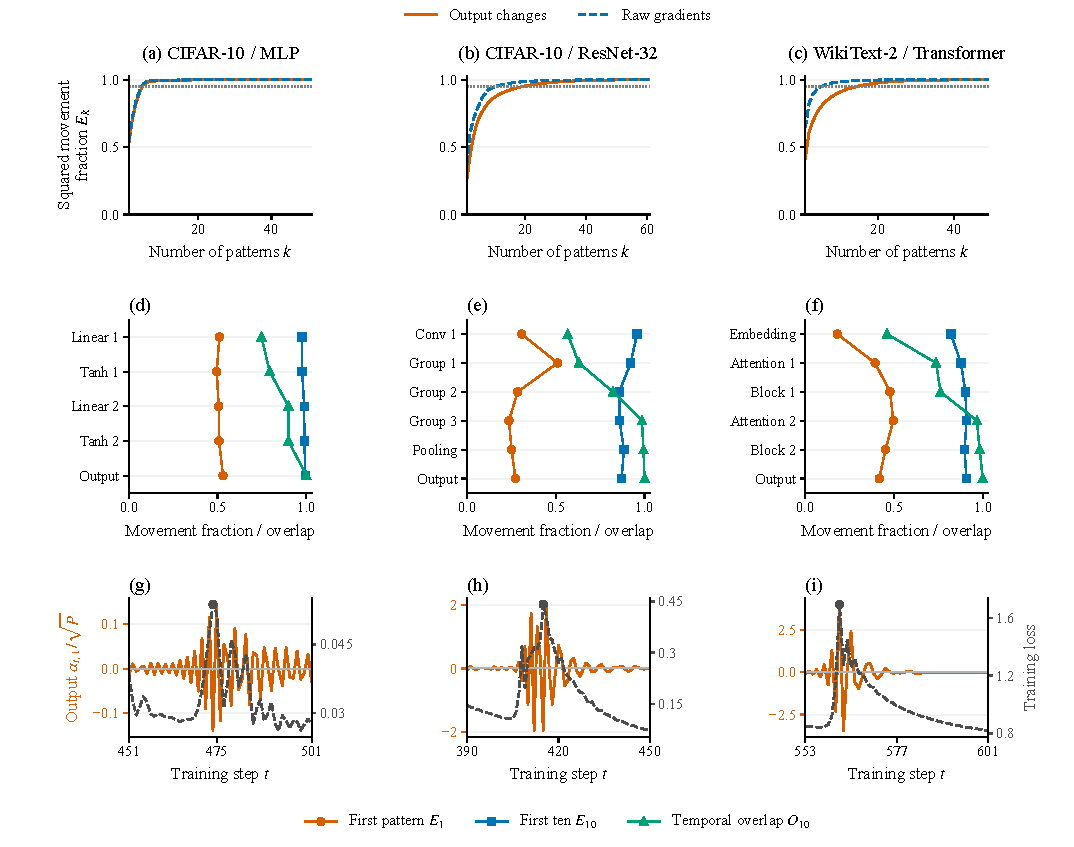
\includegraphics[width=\textwidth]{figures/01-three-model-temporal-structure.pdf}
\caption{Patterns and timing of representation movement in the same windows as Fig.~\ref{fig:trace-motion}, containing 51/61/49 changes. Top: cumulative fraction of squared movement for output changes and for the raw gradients used by those updates; the dotted line marks 95\%. Middle: each site's fraction in its first pattern ($E_1^\ell$) and first ten ($E_{10}^\ell$), and temporal overlap with the output ($O_{10}$). Bottom: signed coefficient of the leading output pattern, divided by $\sqrt P$ to express its coordinate RMS scale. A coefficient crossing zero reverses direction along that fixed pattern. Energy, temporal overlap, and signed motion answer different questions; none alone establishes causal transmission through a layer.}
\label{fig:trace-structure}
\end{figure*}

Figure~\ref{fig:trace-structure} asks whether these changes repeatedly
use a small set of patterns. The top row shows concentration of squared
movement in the leading output modes, alongside the corresponding
gradient decomposition. Concentration can reflect both repeated
directions and a few large changes; the equal-length and orthogonal
controls in Supplementary Section S4 separate these effects.
The middle row extends the analysis through the network: $E_1^\ell$
and $E_{10}^\ell$ show concentration at each site, whereas $O_{10}$ shows
how much its leading temporal structure is shared with the final output.
The selected ResNet window has stronger temporal agreement toward the
output, with shared structure still extending to the input-side sites.
Finally, the bottom row establishes the back-and-forth component that
energy fractions alone cannot establish. Repeated changes in the sign
of $\alpha_{t,1}^F/\sqrt{P_F}$ show reversal along one fixed output
pattern, and its amplitude shows how strongly that pattern moves.

Together, the two figures and the small retention values characterize
coordinated, approximately low-dimensional functional oscillation in
these windows. The temporal Gram matrix $D_\ell D_\ell^\top$ permits
the analysis without storing all spatial modes; implementation and
numerical checks are in Supplementary Section S4. The resulting
intervention question is whether limiting the magnitude of local
representation changes can reduce loss excursions while preserving
subsequent training progress.
